\documentclass[10pt]{article}
\usepackage[utf8]{inputenc}
\usepackage[T1]{fontenc}
\usepackage{amsmath}
\usepackage{amsfonts}
\usepackage{amssymb}
\usepackage[version=4]{mhchem}
\usepackage{stmaryrd}
\usepackage{graphicx}
\usepackage[export]{adjustbox}
\graphicspath{ {./images/} }

\title{homework and recetation review  }

\author{}
\date{}


\begin{document}
\maketitle

homework 6 question 1. (Spam detector) In order to build a spam classifier, we gather the following data. Each row is an email. The first column indicates whether it is spam or not. The remaining columns indicate whether it contains $(\boldsymbol{\checkmark})$ or not $(\boldsymbol{X})$ the word on top.
\begin{tabular}{|c|c|c|c|c|}
\hline & Miracle & Alternative & Medicine & Basketball \\
\hline Spam & $\checkmark$ & $\checkmark$ & $\checkmark$ & $\checkmark$ \\
\hline Not spam & $\boldsymbol{x}$ & $\boldsymbol{x}$ & $\checkmark$ & $\checkmark$ \\
\hline Spam & $\checkmark$ & $\boldsymbol{x}$ & $\boldsymbol{x}$ & $\boldsymbol{x}$ \\
\hline Not spam & $\boldsymbol{x}$ & $\checkmark$ & $\boldsymbol{x}$ & $\boldsymbol{x}$ \\
\hline Spam & $\checkmark$ & $\boldsymbol{x}$ & $\boldsymbol{x}$ & $\boldsymbol{x}$ \\
\hline Not spam & $\boldsymbol{x}$ & $\checkmark$ & $\boldsymbol{x}$ & $\checkmark$ \\
\hline Spam & $\checkmark$ & $\boldsymbol{x}$ & $\boldsymbol{x}$ & $\boldsymbol{x}$ \\
\hline Spam & $\boldsymbol{x}$ & $\checkmark$ & $\checkmark$ & $\boldsymbol{x}$ \\
\hline Not spam & $\checkmark$ & $\checkmark$ & $\boldsymbol{x}$ & $\checkmark$ \\
\hline Not spam & $\boldsymbol{x}$ & $\boldsymbol{x}$ & $\checkmark$ & $\checkmark$ \\
\hline
\end{tabular}
We use a Bernoulli random variable $\tilde{y}$ to model whether the email is spam $(\tilde{y}=1)$ or not $(\tilde{y}=0)$, and a four-dimensional random vector $\tilde{x}$ to indicate whether the $i$ th word is $(\tilde{x}[i]=1)$ or $\operatorname{not}(\tilde{x}[i]=0)$ in the email for $i \in\{1,2,3,4\}$.\\\\
(a) Your friend recommends that you estimate the conditional pmf of $\tilde{y}$ given $\tilde{x}$ and then maximize it to produce your estimate. What is the problem with this approach?
\begin{itemize}
    \item this will not work as there are $2^4=16 $ parameters to estimate from data. 
\end{itemize}
(b) Apply naive Bayes to classify an email that reads I hurt my foot playing basketball. Can you get me some medicine?
\begin{itemize}
    \item let the message containign the words we are intrested in be an rv $x=(x_1,x_2,x_3,x_4)$
    \item we would like $p(s=1|x=x)=\frac{P(x=1,s=1)}{P(x=x)}=\frac{P(x=x|s=1)P(s=1)}{P(x=x|s=1)P(s=1)+P(x=x|s=0)P(s=0)}$
    \item so the x in question in this problem is $x=\begin{pmatrix}
        0\\0\\1\\1
    \end{pmatrix}$
    \item the naive bayes estimator assumes that $x_i,x_j$ are conditionally independint given the class in this case spam 
    \item thus we can express $p(s=1|x=x)=\frac{P(x=1,s=1)}{P(x=x)}=\frac{P(x=x|s=1)P(s=1)}{P(x=x|s=1)P(s=1)+P(x=x|s=0)P(s=0)}=\frac{P(x_1=0|s=1)P(x_2=0|s=1)P(x_3=1|s=1)P(x_4=1|s=1)}{P(x_1=0|s=1)P(x_2=0|s=1)P(x_3=1|s=1)P(x_4=1|s=1)+P(x_1=0|s=0)P(x_2=0|s=0)P(x_3=1|s=0)P(x_4=1|s=0)}$
    \item we can see that $P(s=1)=\frac{5}{10}$ 
    \item we can also see that for example $P(x_1=0|s=1)=\frac{1}{5}$ and $P(x_1=1|s=0)=\frac{4}{5}$
    \item the rest of this problem is just computation 
\end{itemize}


(c) Apply naive Bayes to classify an email that reads This alternative medicine is amazing, send us all your money! Explain what shortcoming of the naive Bayes classifier is illustrated by this example.
\begin{itemize}
    \item the naive bayes assumes condtional Independence between $x_i,x_j$ given c thus it does not really model there interactions and in a case like this clearly that conditional Independence does not hold. ie naive bayes ignores dependinceis between words in an email 
\end{itemize}


Homework 6 question 3: A company that makes mobile phones wants to model the sales of a
new model they have just released. At the moment 90 precent of the phones are in stock,
10 percent  have been sold locally and none have been exported. Based on past data, the
company determines that each day a phone is sold with probability 0.2 and exported
with probability 0.1. We define the following time-homogeneous Markov chain with three
states to model this: (there is a markov chain diagram on the homeowrk so look that up if you want) 
\\ a.  What is the limit of the state vector $\pi_i$ as i aproaches infinity
\begin{itemize}
   \item we can write our transition matrix $T\in \mathbb{R}^{3}$ as $T=$\begin{pmatrix}1,&.1,&0\\0,&.7&,0\\0,&.2,&1
    \end{pmatrix}
    \item we can also write our given intitial state as $\pi_0=\begin{pmatrix} 0\\.9 \\.1 \end{pmatrix}$
    \item so recall that the long term behavior of a matrix can be expressed as $lim_{i\rightarrow\infty}\pi_i=T^{i-1}pi_1=(Q\Lambda Q^{-1})^{i-1}\pi_1=(Q\Lambda^{i-1} Q^{-1})\pi_1$ as Q are orthonormal matrcies of the eigen vectors of T thus raising them to a power keeps them the same and as $\Lambda$ is diagnol raising it to teh power is the same as writing 
    $lim_{i\rightarrow\infty}\pi_i=T^{i-1}pi_1=(Q\Lambda Q^{-1})^{i-1}\pi_1=(Q\Lambda^{i-1} Q^{-1})\pi_1=Q\begin{pmatrix}\lambda^i,&.0,&0\\0,&&\lambda_2^i&,0\\0,&0,&\lambda_3^i
    \end{pmatrix}Q^{-1}$ \begin{pmatrix} 0\\.9 \\.1 \end{pmatrix} 
    \item our matirx T has eigen values $\lambda_1=1,\lambda_2=1\lambda_3=.87$ so at teh limit we will get  $lim_{i\rightarrow\infty}\pi_i=T^{i-1}pi_1=(Q\Lambda Q^{-1})^{i-1}\pi_1=(Q\Lambda^{i-1} Q^{-1})\pi_1=Q\begin{pmatrix}1,&.0,&0\\0,&1&,0\\0,&0,&0
    \end{pmatrix}Q^{-1}$ \begin{pmatrix} 0\\.9 \\.1 \end{pmatrix}=\begin{pmatrix} 0\\.7 \\.3 \end{pmatrix} this makes intuitive sense as non of the phones remain in stock 70 percent are solid domestically and .3 are sold abroad
    \item note that the value of our terminal state crucially depends on the value of our int ital state.
\end{itemize}
recitation 7 question 1 1. Consider the Markov chain with three states, $S=\{1,2,3\}$, that has the following transition matrix
$$
T=\left[\begin{array}{ccc}
1 / 2 & 1 / 3 & 1 / 2 \\
1 / 4 & 0 & 1 / 2 \\
1 / 4 & 2 / 3 & 0
\end{array}\right]
$$
If we know $P\left(X_1=1\right)=P\left(X_1=2\right)=\frac{1}{4}$.\\ 
(a) Compute $P\left(X_1=3, X_2=2, X_3=1\right)$\begin{itemize}
    \item the wordinf of this is a bit dumb but we are givin an intial state vector $\pi_1=\begin{pmatrix}
        .25\\.25\\.5
    \end{pmatrix}$ \item then we can model $P(x_1=3,x_2=2,x_3=1)=P(x_1=3)P(x_2=2|x_1=3)P(x_3=1|x_2=2)$ by the markov proerty 
    \item we know from our state vector that $P(x_1=3)=.5$ and can find the other two values from our t matrix yielding $P(x_1=3,x_2=2,x_3=1)=P(x_1=3)P(x_2=2|x_1=3)P(x_3=1|x_2=2)=.5(.5)(.33)$ 
\end{itemize}
(b) Compute $P\left(X_1=3, X_3=1 \mid X_2=2\right)$
\begin{itemize}
    \item here we want to find $P(x_1=3,x_3=1|x_2=2)=\frac{P(x_1=3,x_2=2,x_3=1)}{P(x_2=2)}=\frac{P(x_1=3,x_2=2,x_3=1)}{\Sigma_{a=1}^{3}P(x_1=a)P(x_2=2|x_1=a)}=\frac{.5(.5)\frac{1}{3}}{(.25)(.25)+(.25)(0)+(.5)(.5)}=\frac{4}{15}$
    \item notice here that we only need to condtion over the first state in the denomiator as we are mkaing no assertions about the third state
\end{itemize}
recetation 7 question 2. In genetics, one method for identifying dominant traits is to pair a specimen with a known hybrid. Their offspring is once again paired with a known hybrid, and so on. In this way, the probability of a particular offspring being purely dominant, purely recessive, or hybrid for the trait is given by the table below.
\begin{tabular}{cccc}
\hline & Child Dominant & Child Hybrid & Child Recessive \\
\hline Parent Dominant & $0.5$ & $0.5$ & 0 \\
\hline Parent Hybrid & $0.25$ & $0.5$ & $0.25$ \\
\hline Parent Recessive & 0 & $0.5$ & $0.5$ \\
\hline
\end{tabular}
(a) If we wanted to model this as a discrete state Markov chain, what is the transition matrix?
\begin{itemize}
    \item the transiton matrix must have colomns that sum to one so it is the transpose of the table. 
\end{itemize}
(b) Compute the eigendecomposition of the transition matrix and use this to discuss how the state vector will converge over time.
\begin{itemize}
    \item we end up with eigenvalues $\lambda_1=0,\lambda_2=.5,\lambda_3=0$
    \item this means that in the limit or $\delta$ matrix will have entery 1,1 as 1 and zeros everyhwere else. 
    \item thus we know that the long term distrobution of our state vector will be completly determined by our first eigenvector. 
\end{itemize}
recetation 7 question 3
\\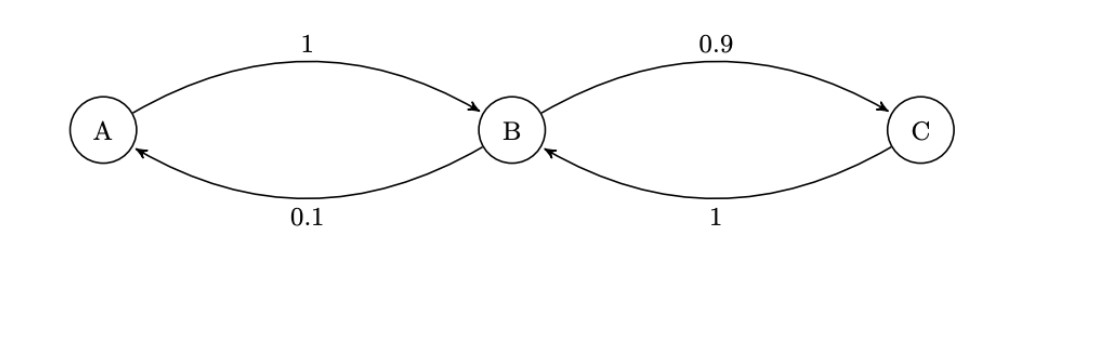
\includegraphics[width=15cm]{final practice/recetation_7_quetion_3.jpg}
\item here we get a matrix t=$\begin{pmatrix}
    .5&.25&0\\.5&.5&.5\\0&.25&.5
\end{pmatrix}$
\begin{itemize}
\item which ends up having eigenvalues of $\lambda_1=-1,\lambda_2=0,\lambda_3=1$ with accompanying eigenvectors $v_1,v_2,v_3$
\item we can tell that as $v_1$ is of eigenvalue 1, $T^{i}v_1=T$ will hold for any value of i, thus if our intial state is $v_1$ tehn we will always end up at final state $v_1$ and it is a solid state 
\item notice however that as $\pi_i=T^{i}\pi_1=Q\lambda^{i}Q^{-1}=Q=\begin{pmatrix}
    (-1)^{i}&0&0\\0&0&0\\0&0&1^{i}
\end{pmatrix}Q\pi_1$ will osilate depedning on if 0 is even or odd as $-1^{even}=1,(-1)^{odd}=-1$
\item this can be further formalized by textbook therome 4.37 which states that a state vector can be represented as a linear combination of the eigenvalues of our transtion matirx $T\in\mathbb{R}^{DXD}$, $\pi_i\mathbb{R}^d$ 
\item that is as our intial state is a vector in r d we can write it is a linear combination of the orthonomiral eigenvectors of T ($v_1..v_n$) that is  $\pi_q=\Sigma_{i=1}^{d}\alpha_iv_i$
\item than as we discussed earlier $\pi_i=T^{i-1}\pi_1=Q\Lambda^{i-1}Q^{-1}\pi_1=\Sigma_{i=1}^{d}\lambda^{i-1}\alpha_iv_i$
\item and as we discussed above $\lambda_1=-1$ so $\pi_i=T^{i-1}\pi_1=Q\Lambda^{i-1}Q^{-1}\pi_1=\Sigma_{i=1}^{d}\lambda^{i-1}\alpha_iv_i$ will not converge 
\item so in summary we know that T can reach a stationary distribution equal to $v_3$ if our initial state is $v_3$, but in other cases our long term distrobution will be osilating and thus not reach a terminal state
\end{itemize} 


homework 7 quesiton 1: There’s a spider living on a wall of your living room that has a painting
behind which the spider likes to hide. Figure 1 shows a diagram of the wall; it is 10 feet
high and 10 feet wide.
After observing the spider for a while you determine that (1) it spends twice the time
behind the painting than on the rest of the wall, (2) it never crawls on the painting or
leaves the wall, (3) if it is not behind the painting then it is equally likely to be anywhere
on the wall. Since you cannot see it behind the painting, you assume that when it is there
it is also equally likely to be at any spot.
\\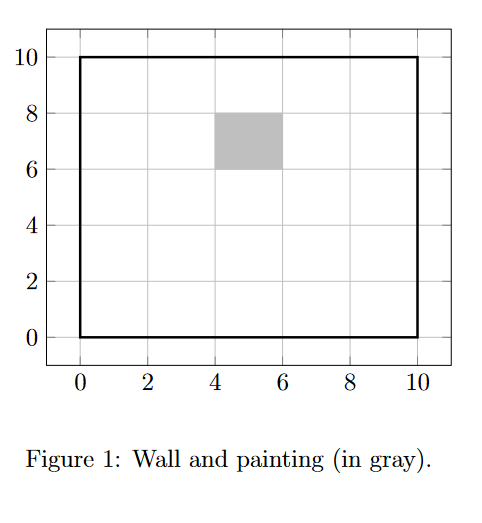
\includegraphics[width=7cm]{final practice/heomwortk 7 question 1.png}


(a) Model the position of the spider as a bivariate random variable and give its pdf.

\begin{itemize}
    \item we know that it spends twice the amount of time behind the painting as elsewhere on the wall. thus hte likeyhood it is behind the painting is $\frac{2}{3}$ we know that the pdf is uniform thus $\frac{2}{3}=(8-6)(6-4)c=(2)(2)(c)=4c$ meaning that $c=\frac{1}{6}$
    \item we know that the total area of the wall is 10X10=100 so the area not behind the painting is 96 meangin that its density is equal to (c) such that $96c=\frac{1}{3}$ and $c=\frac{1}{288}$
    \item we can check this as $\int _6^8\int _4^6\frac{1}{6}dydx\:+\int _0^{10}\int _0^{10}\frac{1}{288}dydx\:-\int _6^8\int _4^6\frac{1}{288}dydx=1$ which is what we ant 
    \item and we know that the spider has 0 lieklyhood of being anywhere else 
\end{itemize}
(b) Compute the pdf of the height at which the spider is located and sketch it.
\begin{itemize}
    \item we are looking for $f_{y|x}(y|x)$ 
    \item here the value depends on x so if x is not in 4,6 but is between 0 and 10 we have $f_{y|x}(y|x)=\int_{0}^{10}f_{x,y}(x,y)dx=\int_{0}^{10}\frac{1}{288}dx=\frac{10}{288}=\frac{5}{144}$
    \item on the other hand if x is between 4,6 then $f_{y|x}(y|x)=\int_{0}^{10}f_{x,y}(x,y)dx=\int_{0}^{6}\frac{1}{288}dx+\int_{6}^{8}\frac{1}{6}dx++\int_{8}^{10}\frac{1}{288}dx=\frac{10}{288}=\frac{8}{288}+\frac{1}{3}=\frac{\left(52\right)}{144}$ 
\end{itemize}
(c) Compute the conditional cdf of the height at which the spider is located, given that
you can see it (i.e. it’s not under the painting) and sketch it
\begin{itemize}
    \item let $s$ be an rv representing wether or not the spider can be seen 
    \item we want to find $f_{y|s}(y|s=1)=\frac{f(y,s=1)}{f(s=1)}$
    \item so first we want to know the liklyhood that the spider can be seen, which is the liklyhood it is not under the painting whcih is given to us as $\frac{1}{3}$ at the start of the problem. 
    \item now we want to think about the joint $f(y,s=1)=\int_{x=0}^{10}f_{x,y,s}(x,y,s=1)dx=\int_{x=0}^{10}f_{s|x,y}(s=1|x,y)f_{x,y}(x,y)dx$
    \item here we are assuming that the spider can be seen 100 percent of the time if they are not behind the painting and 0 percent fo the time if they are behind the painting 
    \item so if y is in [0,6] or [8,10] there are no x values that make it behind the painting and thus $f(y,s=1)=\int_{x=0}^{10}f_{x,y,s}(x,y,s=1)dx=\int_{x=0}^{10}f_{s|x,y}(s=1|x,y)f_{x,y}(x,y)dx=\int_{x=0}^{10}\frac{1}{288}dx=\frac{5}{48}$
    \item if $y\in [6,8]$ there are x values that make the spider behind the painting thus we have $f(y,s=1)=\int_{x=0}^{10}f_{x,y,s}(x,y,s=1)dx=\int_{x=0}^{10}f_{s|x,y}(s=1|x,y)f_{x,y}(x,y)dx=\int_{x=0}^{6}\frac{1}{288}dx+\int_{x=8}^{10}\frac{1}{288}dx=\frac{1}{36}$
    \item now to find the cdf we just integearte it 
    \item assuming that y is less than 6 we get $F_{y|s=1}(a)=\int_{y=0}^{a}f_{y|s}(y)dy=\frac{5y}{48}$
    \item if y is in $[[6,8]$ then we have $F_{y|s=1}(a)=\int_{y=0}^{a}f_{y|s}(y)dy=\frac{30}{48}+\int_{6}^{a}\frac{1}{36}dy=\frac{30}{48}+\frac{8(y-6)}{288}$
    \item  if y is in $[[8,10]$ then we have $F_{y|s=1}(a)=\int_{y=0}^{a}f_{y|s}(y)dy=\frac{30}{48}+\frac{16}{288}+\int_{8}^{a}\frac{5}{48}dy=\frac{30}{48}+\frac{16}{288}+\frac{5(y-8)}{48}$
\end{itemize}
homework 7 question 3. (Sonar) A scientist is trying to determine the depth of the sea at a certain location. She knows that it must be deeper than $5 \mathrm{~km}$ but that is all she knows. To capture this uncertainty she models the depth as uniformly distributed between 5 and $10 \mathrm{~km}$. In order to measure the depth she uses sonar, taking 2 measurements, which we model as two random variables $\tilde{s}_1$ and $\tilde{s}_2$. If the depth is equal to $x$ then each sonar measurement is uniformly distributed between $x-0.25$ and $x+0.25$. The two measurements are conditionally independent given the depth.
\\(a) Compute and sketch the pdf of the first sonar measurement $\tilde{s}_1$.
\begin{itemize}
    \item so here we are looking for $f(s_1)=\int_{x\in X}f(s_1,x)=\int_{x\in X}f(s_1|x)f_x(x)$
    \item we know that x is unfform in 5,10 thus $f_x(x)=\frac{1}{5}$
    \item we know that s1 is unform betwen x-.25 and x+.25  so thus $f_{s_1|x}(s|x)=2$ but only for values within a range of plus or minus .5 x
    \item so lets consider $s_1\in[5,5.25]$ this is equal to $f(s_1)=\int_{x=5}^{10}f(s_1,x)=\int_{x=5}^{10}f(s_1|x)f_x(x)$ but here we know that $f(s_1|x)$ only has non zero probability on the interval $[x-.25,x+.25]$ which can have a range of $[4.75,5.5]$ depedning on the $s_1$ x on the other hand is only defined from 5 to 10
    \item thus our integral only takes non zero probabiltiy when $f(s_1)=\int_{x=5}^{10}f(s_1,x)=\int_{x=5}^{10}f(s_1|x)f_x(x)=\frac{5}{s_1+.25}\frac{1}{5}2dx=\frac{2}{5}\int_{5}^{s_1+.25}dx=\frac{2}{5}(s_1+.25-5)=\frac{2}{5}(s_1-4.75)$
    \item on the other hand when $s_1$ is in the range [5.25,9.75] we have no issues and get  $f(s_1)=\int_{s_1-.25}^{s_1+.25}\frac{2}{5}dx=(s_1+.25-s_1+.25)\frac{2}{5}=\frac{1}{5}$
    \item finally if $s_1$ is in [9.75,10] by the same arugment as in case a we cna see taht  $f(s_1)=\int_{9.75}^{s_1+.25}\frac{2}{5}dx=\frac{2}{5}(s_1-9.5)$
\end{itemize}
(b) compute the conditional pdf of the depth conditioned on the measurements being
equal to 7 km and 7.1 km.
\begin{itemize}
    \item we are looking for $f_{x|s_1,s_2}(x|s_1,s_2)=\frac{f(x)f(s_1|x)f(s_2|x)}{\int_{x}f(s_1)f(s_2)f(x)}dx$
    \item this value is only non zero if s is in [6,85,2.75] since at that value both 7,and 7.1 are within plus or minus .5 of x
    \item thus we can see that $f_{x|s_1,s_2}(x|s_1,s_2)=\frac{f(x)f(s_1|x)f(s_2|x)}{\int_{x}f(s_1)f(s_2)f(x)}dx=\frac{2*2*\frac{1}{5}}{\int_{6.85}^{7.25}}2*2*\frac{1}{5}=\frac{5}{2}$
    \item and zero elsewhere 
\end{itemize}
(c) Compute the joint pdf of the two sonar measurements  ̃s1 and  ̃s2. Are the two
measurements independent? Justify your answer mathematically and explain it in-
tuitively
\begin{itemize}
    \item $f_{s_1,s_2}(s_1,s_2)=\int_xf(s_1,s_2,x)=\int_{x}f(x)f(s_1|x)f(s_2|x)$ by conditional Independence 
    \item we know that both $f(s_1|x),f(s_2|x)$ are only non zero if $|s_1-s_2|\leq .5$ that is if they are within .5 of each other and x is only non zero between 5 and 10
    \item thus we can define $f_{s_1,s_2}(s_1,s_2)=\int_xf(s_1,s_2,x)=\int_{max(5,s_1-.25,s_2-.25)}^{min(10,s_1+.25,s_2+.25)}f(x)f(s_1|x)f(s_2|x)dx=$ 
\end{itemize}


recetation 8 question 1. (2D Gaussian) Let us consider a two-dimensional Gaussian random vector $(\tilde{a}, \tilde{b})$ with zero mean and covariance matrix
$$
\Sigma:=\left[\begin{array}{ll}
1 & \rho \\
\rho & 1
\end{array}\right],
$$
where $\rho$ is a parameter and $-1 \leq \rho \leq 1$, which we call the correlation coefficient of the vector. Hint: the joint pdf of a Gaussian random vector $\tilde{x} \sim \mathcal{N}(\mu, \Sigma)$ is
$$
f_{\tilde{x}}(x)=\frac{1}{\sqrt{(2 \pi)^d|\Sigma|}} \exp \left(-\frac{1}{2}(x-\mu)^T \Sigma^{-1}(x-\mu)\right),
$$
where $\mu \in \mathbb{R}^d$ and $\Sigma \in \mathbb{R}^{d \times d}$.\\
(a) Compute the joint pdf $f_{\tilde{a} \tilde{b}}(a, b)$;
\begin{itemize}
    \item this part is just computational 
    \item $det(A)$ for a two d matrix is ad-cd so in this case our det is $1-\ro^2$
    \item our x=(a,b)
    \item our $\mu=(0,0)$
    \item working this out gives us a pdf of $$
=\frac{1}{\sqrt{2 \pi}} \exp \left(-\frac{a^2}{2}\right) \frac{1}{\sqrt{2 \pi\left(1-\rho^2\right)}} \exp \left(-\frac{(b-\rho a)^2}{2\left(1-\rho^2\right)}\right) .
$$ after we take everything out of matrix and vector form. 

\end{itemize}
(b) Compute the marginal pdf $f_{\tilde{a}}(a)$ and $f_{\tilde{b}}(b)$;
\begin{itemize}
    \item here in order to avoid really messy calculations just apply therome 5.24 on page 33 of chapter 5 of the textbook 
    \item doing this we find that $f_{a}(a)$ is a gausain random vairble
    \item we know that the mean is zero for the problem discripiton 
    \item further we know that it must be teh case that $\sigma_a^2=1$ and $sigma_a*\sigma_b=\ro$ menaing that $\sigma_a=\sigma_b=1$
    \item thus we know that the marginal of a and b are a gausian random vairbles with mean 0 and varinace 1. 
    \item thus $f_(a)(a)=f_(B)(b)=\frac{1}{\sqrt{2\pi}}e^{\frac{-1}{2}}(a^2)$
 \end{itemize}
(c) Compute the conditional pdf $f_{\tilde{b} \mid \tilde{a}}(b, a)$.
\begin{itemize}
    \item by the same therome we can find that the codntional of b given a is a guasian rv with mean = $\rho a$ and standard devation $f_{b|(a)}(b|a=\frac{1}{\sqrt{2\pi}(1-\rho^2)}e^{\frac{-1}{2}}(\frac{(b-\ro a)^2}{1-\ro^2})$
\end{itemize}
1. (Bayesian coin flip) Let us try out another prior for the Bayesian coin flip problem in the notes. We now model the parameter of the Bernouilli as being uniform between $1 / 2$ and 1.
\\(a) Briefly justify the model and compute the probability that the result of the coin flip is heads or tails under this model.
\begin{itemize}
    \item they ask this question in a dumb way they are just asking for the heads proability 
    \item $P(y=1)=\int_{\theta=\frac{1}{2}}^{1}P(y=1,\theta)=\int_{\theta=\frac{1}{2}}^{1}P(y=1|\theta)P(\theta)d\theta=\int_{\theta=\frac{1}{2}}^{1}2(\theta)d\theta=\frac{3}{4}$
    \item doing the same thing for tails we find that $P(y=0)=\frac{1}{4}$
\end{itemize}
(b) After the coin flip we update the distribution of the bias of the coin (i.e. the parameter of the Bernouilli that represents the coin flip) by conditioning it on the outcome. Compute the distribution if the outcome is tails and if the outcome is heads. Sketch any distributions you compute and explain why the drawing makes sense.
\begin{itemize}
    \item the posterior can be computer as $P(\theta|y)=\frac{P(y,\theta)}{P(y)}=\frac{P(y|\theta)P(\theta)}{P(y)}$
    \item then it is just a matter of plugging in values that have akready been comptuer and taking an integral 
    \item the real point is that the posterior adjusts with the observed outcome, but becuase of our priro rit cna never adjust past $\theta=\frac{1}{2}$ so this wil inluince our conclsuions 
\end{itemize}
homework 9 question 1c  A teacher of a class of n children asks their parents to leave a present under the
Christmas tree in the classroom. The day after, each child picks a present at random.
What is the expected number of children that end up getting the present bought by
their own parents? (Hint: Define a random variable  ̃ai that is equal to one when kid
i gets the present bought by their own parents, and to zero otherwise.)
\begin{itemize}
\item we lets deffine an rv $a_i$ which takes on value 1 if child i gets the present their parent bought 
\item we can call the total number of presents $a=a(a_1...a_n)=a_1+...+a_b$
\item so we can see that $E[a]=E[a(a_1..a_n)]=E[a_1...a_n]=E[a_1]+...+E[a_n]$
\item we can see that $E[a_a]=1P(a=1)+0p(a=)=1P(a_i=1)=\frac{1}{n}$
\item thus we have $E[a]=E[a(a_1..a_n)]=E[a_1...a_n]=E[a_1]+...+E[a_n]=\frac{1}{n}+...+\frac{1}{n}=\simga_{i=1}^{n}\frac{1}{n}=\frac{n}{n}=1$
\end{itemize}

recetation 10 question 2
(Expectation) There are $N$ students in a class. The professor decides to pick a student at random every time he asks a question during the lecture. What is the expected number of questions he should ask, so that every student is asked at least one question?
\begin{itemize}
    \item we want to pick each student once. 
    \item think of $a_i$ as the number of questions it takes to pick the $i_th$ unpickes student 
    \item so $a_1$ means that no students have yet been picked thus we have $p_{a_{1}}(x)=1$ as the recipaint of the first quesitn has always never been chosen before 
    \item $a_2$ models how many questions it takes to pick the second unchosen student thus we have $P_{a_2}(x)=(\frac{1}{n})^x\frac{n-1}{n}$
    \itemt his can be extended to the ith unpicked student as $P_{a_n}(x)=(\frac{i+1}{n})^x\frac{n-i-1}{n}$
    \item this overall gives us that $a_i$ has parameter $\frac{n-i-1}{n}$
    \item so we model the total number of questions for all the students to be picked as $a=a_1+a_2...+a_n$
    \item thus we can see $E[a]=e[a_1+...a_n]=E[a_1]+...+E[a_n]$ 
    \item we know that the mean of a geometric rv with parameter $\alpha $is $\frac{1}{\alpha}$
    \item so overall we have $E[a]=e[a_1+...a_n]=E[a_1]+...+E[a_n]=\Sigma_{i=1}^{n}\frac{n-i-1}{n}$
\end{itemize}
question3 receation(Coins and dice) Let $\tilde{y}$ be the number of heads in $\tilde{x}$ tosses of a fair coin, where $\tilde{x}$ is a fair dice roll.
find  $E[\tilde{y} \mid \tilde{x} = x] = \sum_y y \cdot p(y \mid x)$ 
\begin{itemize}
    \item $y|x$ is binomial with parameter $\frac{1}{2}$ item so it's expectation is the conditional mean function $\mu_{y|x}(x)$
    \item thus if we sum over our values of y we get 1.75
\end{itemize}
\\
homework 10 question 2 
We define the conditional variance function $\nu_{\rb \cnd \ra}(a)$ of a random variable $\rb$ given another random variable $\ra$ as the variance of $\rb$ conditioned on the event $\ra = a$. Analogously to the conditional mean, we define the conditional variance $\nu_{\rb \cnd \ra}(\ra)$ of $\rb$ given $\ra$ as the random variable obtained by plugging $\ra$ into the conditional variance function. 
\begin{itemize}
    \item note that the conditional varinace function here is defined as $V_{b|a}(a)=\mu_{b^2|a}(a)-\mu_{b|a}(a)^2$
    \item i'm dont think the proof is nessvary but here is the law of conditoanl varinace $$
\operatorname{Var}[\tilde{b}]=\mathrm{E}\left[\nu_{\tilde{b} \mid \tilde{a}}(\tilde{a})\right]+\operatorname{Var}\left[\mu_{\tilde{b} \mid \tilde{a}}(\tilde{a})\right] .
$$

\end{itemize}

\end{document}